\newpage
\subsection{Indflydelse af basrefleksens længde}
I dette afsnit vil der blive set på, hvordan længden af basrefleksen kommer til, at spille en rolle i kabinettets samlede frekvenskarakteristik. For at holde variabel-kontrol, så bliver der i første omgang kun målt på betydningen af længden, når basrefleksen er placeret på forsiden af kabinettet.

Der ønskes målt på to dele af højtalerkabinettet: Membranen og basrefleksrøret. Dette gøres ved, at placere CLIO-mikrofonen helt op ad membranen eller helt inde i basrefleksrøret. De to målinger kommer måske ikke til, at være helt akustiske adskilte, men dette er en fejlkilde man er nødt til at leve med.

I første omgang måles der kun på selve membranen, når basrefleksen sidder på forsiden. Resultaterne af disse målinger bliver opvejet med de målinger som blev fundet når kabinettet var helt lukket (ingen basrefleks). Resultatet af dette ses nedenfor.
\begin{figure}[H]
	\centering
	\vspace{-12pt}
	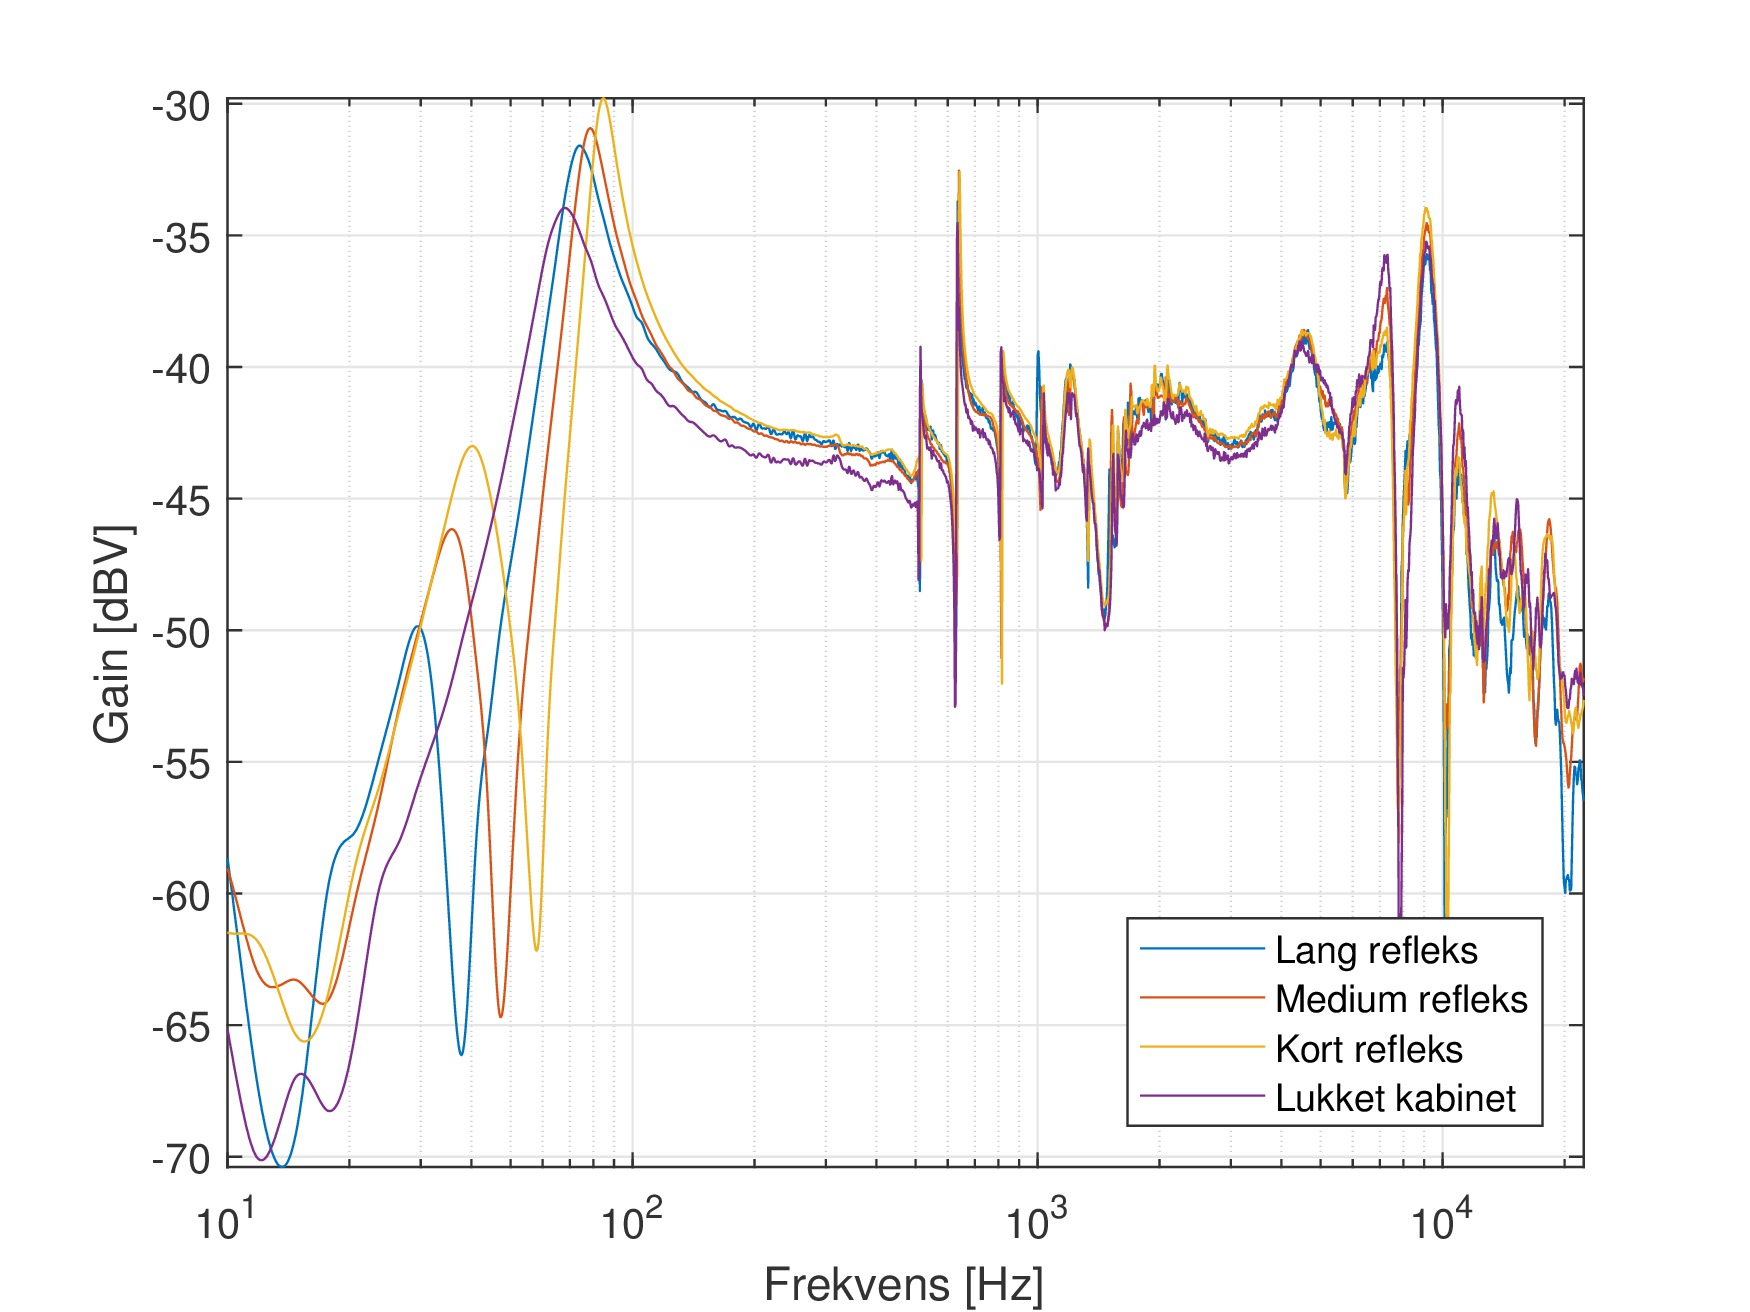
\includegraphics[width=\textwidth]{Billeder/Grafer/BasrefleksLengthMembran}
	\caption{Betydning af basrefleksens længde (målt på membran)}
\end{figure}

Det centrale ved de ovenstående måleresultater er, at der nu forekommer et 'forstærkningsdyk' omkring de lave frekvenser. Samtidig ændres både resonansfrekvensen $f_s$ placering og forstærkningen ved resonansfrekvensen, når der tilføjes en basrefleks eller ændres på længden af basrefleksen.

Det ses på figuren, at jo kortere basrefleksen bliver, jo højere op i både frekvens og forstærkning kommer resonansfrekvensen $f_s$. Samtidig ses det også, at jo længere basrefleksen bliver, jo længere ned i frekvens kommer forstærkningsdykket til at ligge, men at forstærkningen under denne faktisk stiger.

Næste skridt er, at se på selve basrefleksrørets frekvensrespons
\begin{figure}[H]
	\centering
	\vspace{-12pt}
	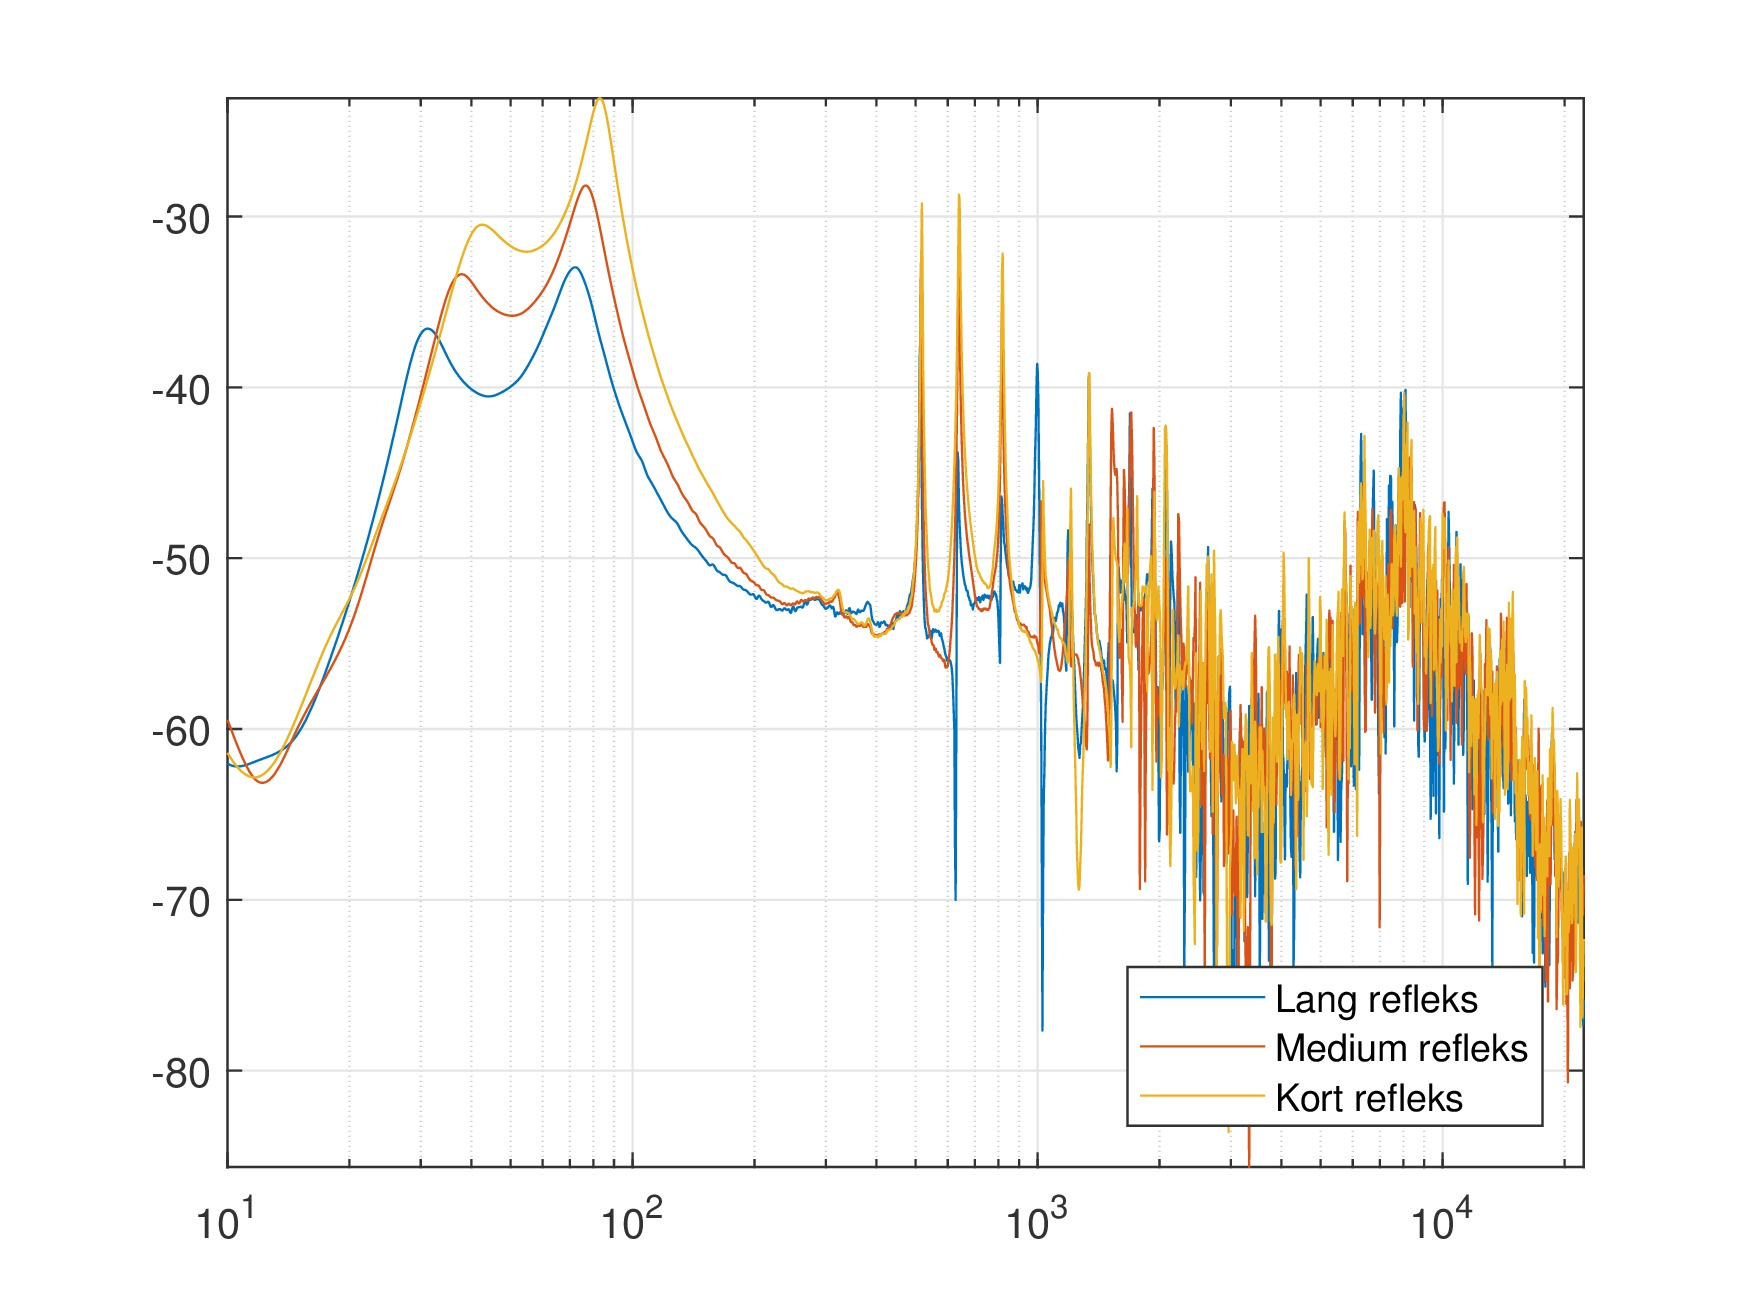
\includegraphics[width=\textwidth]{Billeder/Grafer/BasrefleksLengthTube}
	\caption{Betydning af basrefleksens længde (målt i basrefleks)}
\end{figure}